\cleardoublepage\phantomsection
\phantomsection\mtcaddchapter[Anexo A: información suplementaria]
\FormatoAnexoA

%Agrego las marcas laterales
\AddLabelsAxUno

%Problemas con el tema del fancystyle
\let\originalstyle=\thispagestyle            % Store the command for later reuse.
\def\thispagestyle#1{\fancyfoot[C]{}}       % This clears footer in the center if fancyhdr is in use.
\def\thispagestyle#1{\originalstyle{empty}} % Use this to get blank header+footer, TeXnically it is only \thispagestyle{empty}.
\def\thispagestyle#1{}                       % This line completely ignores the content of the \thispagestyle command.

%Esto cambia el contador de las figuras para que coloque la letra del apendice
\renewcommand\thefigure{A.\arabic{figure}} 

\chapter*{Anexo A: información suplementaria}
  
  
    Se agregan en éste anexo los gráficos, imágenes y espectros que fueron apartados del cuerpo principal de la tesis. 

    \subsection*{Correspondientes al capitulo \ref{chap:Mesoporosos}}

    
    \begin{figure}[th]
		 	   	    \begin{subfigure}[t]{0.49\textwidth}
			       	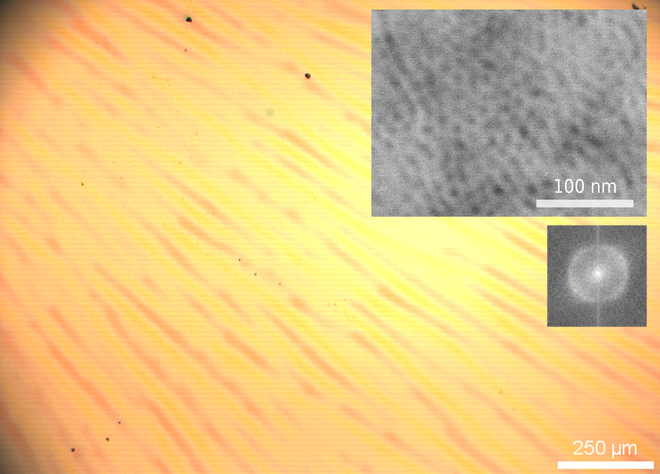
\includegraphics[width=\textwidth]{Imagenes/Au_EtF127-Combinada.jpg}
			   		\end{subfigure}
			   		\begin{subfigure}[t]{0.49\textwidth}
			   	    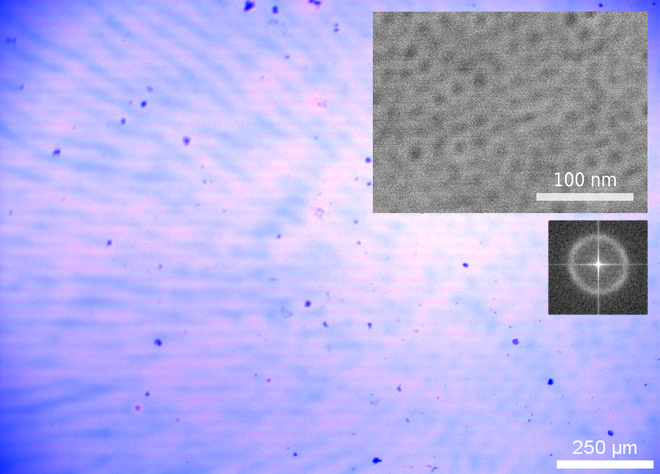
\includegraphics[width=\textwidth]{Imagenes/Si_EtF127-Combinada.jpg}
			   		\end{subfigure}
					 \caption[Microscopías \pdmF\space tratamiento simplificado.]{Microscopías ópticas para \pdmF\space sintetizadas por el tratamiento simplificado. Izquierda: sobre sustrato de Au. Derecha: sobre sustrato de Si. En los respectivos recuadros se observa el detalle por MEB del arreglo nanoporoso.}
					 \label{fig:Microscopia_F127_simplificado}	
				     \end{figure}		

	\begin{figure}[th]
 	   	    \begin{subfigure}[t]{0.49\textwidth}
	       	\includegraphics[width=\textwidth]{Imagenes/Au_EtCTAB-Combinada.jpg}
	   		\end{subfigure}
	   		\begin{subfigure}[t]{0.49\textwidth}
	   	    \includegraphics[width=\textwidth]{Imagenes/Si_EtCTAB-Combinada.jpg}
	   		\end{subfigure}
			 \caption[Microscopías \pdmC\space tratamiento simplificado.]{Microscopías ópticas para \pdmC\space sintetizadas por el tratamiento simplificado. Observese las grietas presentes cuando se sintetiza sobre Au (izquierda), mientras que sobre Si las \pdmC\space no presentan rupturas ni discontinuidades.}
			 \label{fig:Microscopia_CTAB_simplificado}	
		     \end{figure}	

  \let\thispagestyle=\originalstyle